
\section{Systèmes embarqués}

\subsection{Architecture}

\vspace*{-20pt}

\begin{definition}{}
Un \textbf{système informatique embarqué} est un système de traitement de l'information autonome ne possédant pas d'entrée et sortie standard comme le clavier et l'écran. Les informations sont reçues de l'extérieur par le biais de \textbf{capteurs}, elles sont traités par un \textbf{processeur} et selon le programme du système des actions physiques peuvent être déclenchées avec des \textbf{actionneurs}. Les capteurs sont des  \textbf{périphériques d'entrée} et les actionneurs des  \textbf{périphériques de sortie}.

\end{definition}


Les signaux capturés sont \textbf{analogiques}, \ie{} analogues au phénomène : par exemple la rotation de l'axe d'un anémomètre qui mesure la vitesse du vent sur une station météo. Pour être traités par le processeur, ils sont numérisés \ie{} transformés en un nombre fini d'informations codées par des 0 et des 1 par \textbf{échantillonnage} (nombre fini de relevés)  et \textbf{quantification} (nombre fini de valeurs possibles).

Les \textbf{microcontrôleurs} sont des circuits intégrés qui concentrent  une mémoire, un processeur, des entrées-sorties comme un ordinateur mais se caractérisent par une miniaturisation accrue, une plus faible consommation électrique et des performances moindres, mais suffisantes pour des applications toujours plus nombreuses avec les progrès techniques.

Les systèmes informatiques embarqués sont utilisés dans tous les domaines : l'industrie (robots), le transport (avionique, automobile, métro \ldots ), la médecine (pacemakers, imagerie \ldots), la maison (domotique, appareils ménagers \ldots), les télécommunications (téléphonie \ldots), le monde du travail (contrôle d'accès \ldots), les loisirs (vélo électrique \ldots).

On parle  d'\textbf{informatique ubiquitaire} pour désigner cette omniprésence de l'informatique dans notre environnement. 

Les ordiphones modernes  ne sont pas des microcontrôleurs mais des ordinateurs miniatures bien plus puissants que  les systèmes de guidage des premières missions Apollo qui ont amené l'homme sur la lune !  Ils sont dotés de nombreux capteurs.


\begin{center}
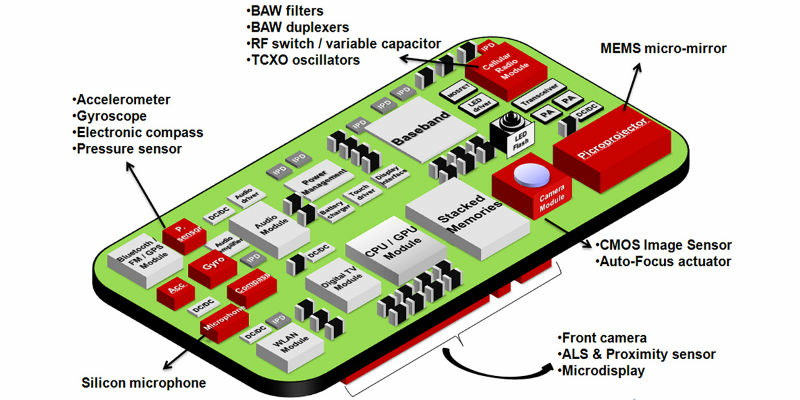
\includegraphics[scale=0.5]{smartphone.png}

{\itshape Source :  flickr / Intel Free Press }
\end{center}



\subsection{Programmation}


\begin{center}
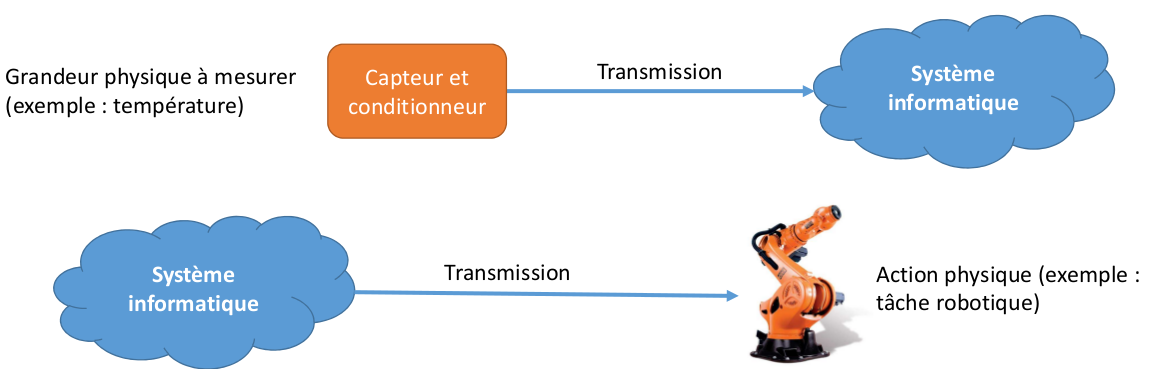
\includegraphics[scale=0.4]{systeme_embarque.png}

{\itshape \small Source : Yassine Haddab Université de Montpellier}
\end{center}


\begin{methode}{}
Un algorithme de contrôle  fréquent sur un système informatique embarqué consiste en une boucle infinie où s'enchaînent capture d'événements par les émetteurs, traitement puis action par les actionneurs.  
\begin{lstlisting}[style=compil]
Initialiser les actionneurs à leur position de départ
Tant que Vrai 
	Lire les informations des capteurs
	Traiter ces informations
	Calculer des informations sur les actionneurs
	Transmettre ces informations aux actionneurs
\end{lstlisting}

\end{methode}



\subsection{QCM type E3C2}


\begin{exerciceB2}{}
Pour chaque question, sélectionner l'unique réponse correcte.

\begin{enumerate}
	\item Identifier parmi les éléments suivants celui qui n'est pas un capteur.

\begin{multicols}{2}
\begin{enumerate}
	\item haut-parleur
	\item caméra
	\item accéléromètre
	\item microphone

\end{enumerate}
\end{multicols}
	
	\item Parmi les éléments suivants, lequel est un capteur ?
	
\begin{multicols}{2}
\begin{enumerate}
\item un bouton poussoir
\item un moteur
\item une diode électroluminescente
\item un afficheur à cristaux liquides

\end{enumerate}
\end{multicols}

\item On réalise une petite station météo.

Quel composant est un capteur ?

\begin{multicols}{2}
\begin{enumerate}
\item l'afficheur LCD
\item l'écran de l'ordinateur
\item la LED
\item le thermomètre
\end{enumerate}
\end{multicols}

\item Parmi les dispositifs d'entrée et de sortie suivants, lequel est
uniquement un capteur ?

\begin{multicols}{2}
\begin{enumerate}
\item la diode
\item l'écran tactile
\item le thermomètre
\item le moteur pas à pas

\end{enumerate}
\end{multicols}
\end{enumerate}

\end{exerciceB2}

 
\section{Interface Homme Machine}

\begin{definition}{}
Une \textbf{Interface Homme Machine} est un ensemble de moyens physiques (boutons, manettes) ou logiciels (interface graphique) qui permettent à un humain d'échanger des informations avec une machine.

Les moyens matériels permettant l'interaction sont appelés \textbf{périphériques} : on distingue les \textbf{périphériques d'entrée} ou de \textbf{sortie}. 

\href{https://interstices.info/50-ans-dinteraction-homme-machine-retours-vers-le-futur/}{Douglas Engelbart} est un des pionniers des IHM en informatique avec son système \textit{NLS} qui introduit  la première souris.
\end{definition}



\begin{exerciceB}{}

Compléter la légende de la figure ci-dessous représentant différents composants et périphériques d'un ordinateur :


\begin{center}
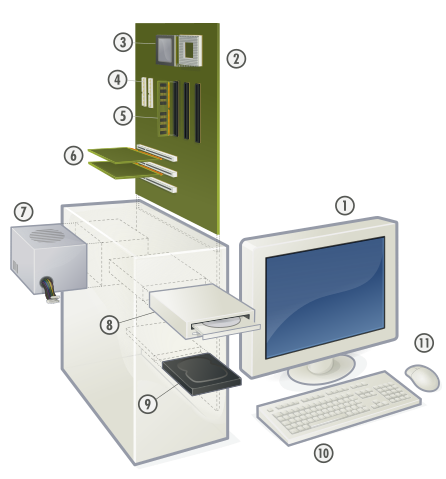
\includegraphics[scale=0.6]{446px-Personal_computer,_exploded_4.svg.png}

\medskip

{\itshape Source : Gustavb / CC BY-SA (http://creativecommons.org/licenses/by-sa/3.0/)}
\end{center}

\end{exerciceB}


\subsection{Fiabilité et sécurité}

\begin{itemize}[label=\ding{43}]

	\item La \textbf{sûreté} est la garantie qu'un système fait ce qu'il doit faire et ne fait pas ce qu'il ne doit pas faire. Les programmes des systèmes embarqués doivent parfois s'exécuter avec des contraintes fortes (manque de ressource, temps de réaction très rapide) et  ils ne sont pas toujours développés avec la rigueur nécessaire. Les bugs sont donc fréquents. Parfois bénins (une mauvaise gestion des années bissextiles a provoqué l'arrêt  du lecteur MP3 Zune de Microsoft le 31/12/2008, ils peuvent avoir  a des conséquences  dramatiques : les bugs  du Therac 25 (appareil de radiographie) ou du contrôle moteur sur les Toyota Camry ont provoqué plusieurs morts.
	
	\item La \textbf{confidentialité} est une problématique majeure des systèmes embarqués qui collectent des données personnelles sur leurs utilisateurs, comme par exemple les cartes électroniques de transport comme le pass Navigoo ou la carte Técély.
	
	\item La \textbf{sécurité}  est souvent un point faible des systèmes embarqués, qui manquent de ressources matérielles, ont des cycles de vie long sans mise à jour et mettent en jeu des modes de communication sans contact particulièrement vulnérables. 
	
Par exemple, une voiture ne peut démarrer que si la carte de démarrage se trouve à proximité car la carte et la voiture partagent un secret commun permettant de déverrouiller le système antidémarrage. \href{https://interstices.info/la-securite-des-systemes-informatiques-ubiquitaires/}{L'attaque par relais} permet  de déjouer ce  protocole  en relayant la communication : un pirate se trouve près de la voiture et l'autre près de la carte et par un leurre technologique ils font croire aux deux parties qu'elles sont à proximité.  Tous les systèmes embarqués qui communiquent sans contact (carte bancaire, carte d'accès \ldots) sont vulnérables à cette attaque.
	
\begin{center}
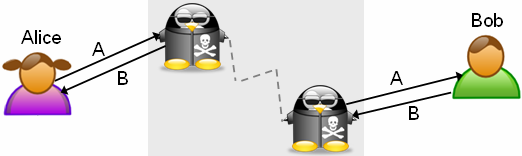
\includegraphics[scale=0.5]{Attaque_par_relais.png}

{\itshape \small Source : Image : Martial Régereau [CC BY-SA 3.0], via Wikimedia Commons}
\end{center}
	
\end{itemize}



\subsection{QCM type E3C2}

\begin{exerciceB2}{}
Pour chaque question, sélectionner l'unique réponse correcte.

\begin{enumerate}
	\item Lequel de ces objets n'est pas un périphérique ?

\begin{multicols}{2}
\begin{enumerate}
	\item le clavier
	\item une clé USB
	\item la carte graphique
	\item la carte mère

\end{enumerate}

\end{multicols}

	\item Lequel de ces périphériques n'est pas un périphérique d'entrée ?

\begin{multicols}{2}
\begin{enumerate}
	\item le moniteur
	\item le clavier
	\item la souris
	\item le scanner

\end{enumerate}

\end{multicols}

\end{enumerate}


\end{exerciceB2}

\section{Objets connectés}

\subsection{Internet des objets}

\vspace*{-20pt}

\begin{definition}{}
Un \textbf{objet connecté} est un système informatique embarqué disposant d'une connexion à un réseau local ou à L'Internet. 

Les Interfaces Homme Machine des objets connectés sont souvent des applications Web disponibles sur Smartphone.


\end{definition}




\begin{center}
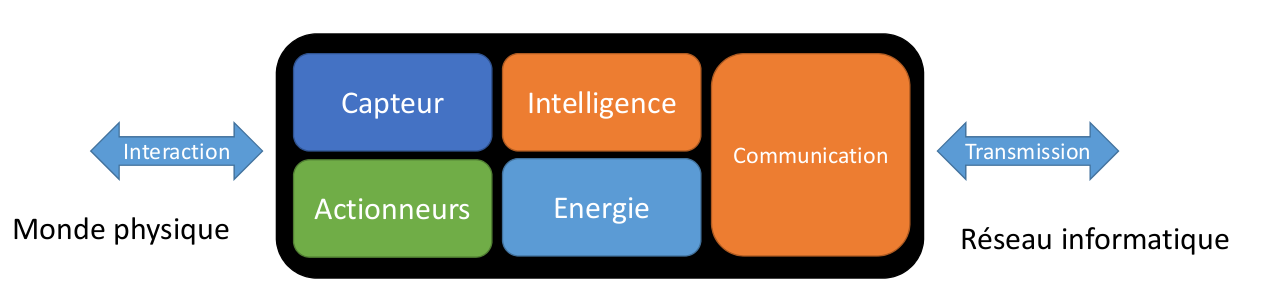
\includegraphics[scale=0.4]{objet-connecte.png}

{\itshape \small Source : Yassine Haddab Université de Montpellier}
\end{center}

Avec la baisse des coûts des microcontrôleurs et des puces Wifi, les objets connectés se multiplient. On peut en fabriquer facilement à partir de cartes Arduino, de Raspberry Pi ou de cartes Wifi ESP8266.
Actuellement, il existe plus d'objets que d'humains connectés à Internet et leur nombre va augmenter fortement dans les prochaines années avec la baisse de coût des . On parle d'\texttt{IOT} pour \href{https://fr.wikipedia.org/wiki/Internet_des_objets}{Internet Of Things} pour désigner l'ensemble des objets connectés à l'Internet.

On estime à 50 milliards le nombre d’objets connectés en 2020.


\subsection{Fiabilité et sécurité}

Les objets connectés permettent d'ajouter de l'intelligence dans notre environnement à tous les niveaux : le corps (mes indicateurs de santé, ma nourriture), la maison(appareils, système de chauffage), les réseaux (électrique, de circulation), les transports (véhicules autonomes), la prévention des risques (incendies) \ldots De plus la collaboration entre objets connectés, leur connexion à des bases de données en ligne, augmente considérablement leur puissance même si chaque objet a des ressources matérielles limitées.

Néanmoins les vulnérabilités des systèmes embarqués sont amplifiées s'ils sont connectés.

\href{https://fr.wikipedia.org/wiki/Cyberattaque_de_2016_contre_Dyn}{La cyberattaque d'un  serveur DNS majeur} par des milliers de caméras de surveillance transformées en bots, a gravement perturbé Internet en Octobre 2016. La prise de contrôle à distance par des hackers de la \href{https://www.wired.com/2015/07/hackers-remotely-kill-jeep-highway/}{Jeep Cherokee} en 2015 ou des failles détectées dans des pacemakers sont des exemples parmi bien d'autres illustrant le fait que la révolution  de l'internet des objets ne pourra se faire sans des progrès sur le plan de leur sécurité.

Enfin  la moisson de données personnelles que  peuvent collecter des objets connectés comme les assistants personnels proposés par les \href{https://fr.wikipedia.org/wiki/GAFAM}{GAFAM}  doit absolument être contrôlée.

